\section{Discussion}
\subsection{Linear Regression}
\begin{figure}[H]
    \centering
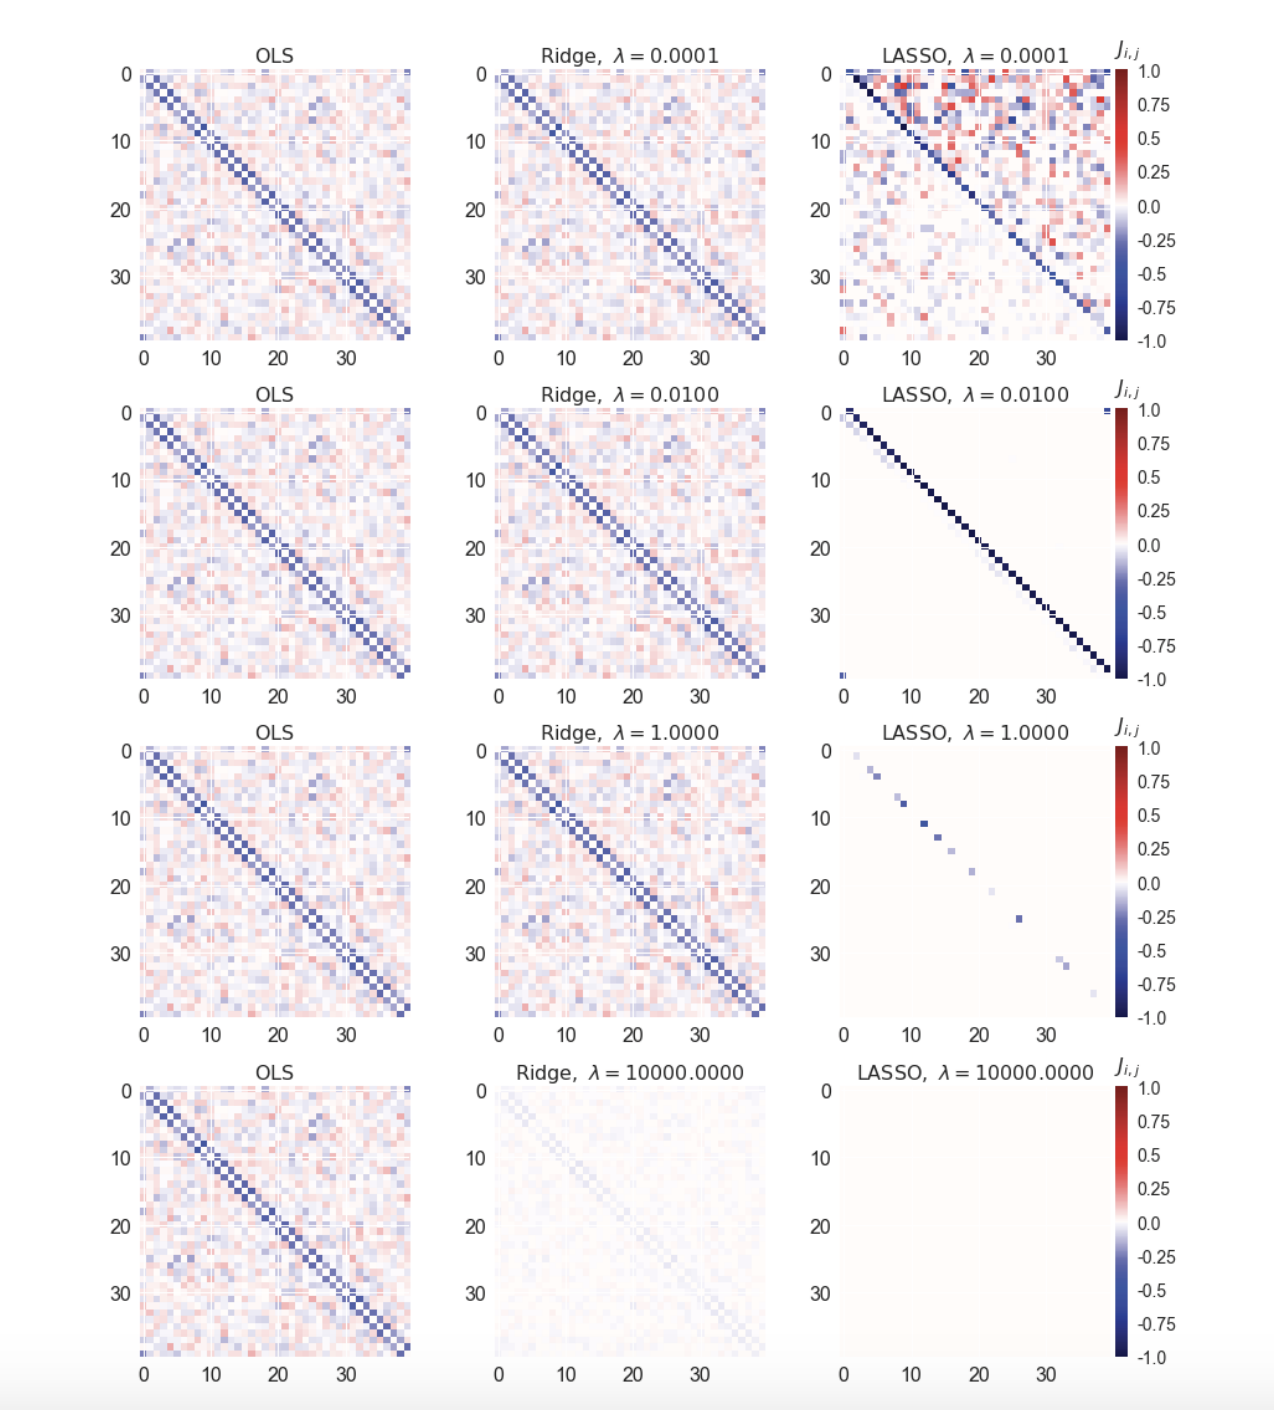
\includegraphics[width = 0.7\paperwidth]{figures/Regression_metha_article.png} 
\caption{Figures from article ~\cite{HighBias} shows similarities to the ones generated by our regression models.} 
\label{fig:regression-mehta-article}
\end{figure}
Based on figures \ref{fig:regression-mehta} and 
\ref{fig:regression-mehta-article}, we see that the figure in article 
~\cite{HighBias} is similar to our own figures. 
Compared to the plots in the article our plots shows less noise, 
and some other small differences, but we see that the tendencies are the same.

Looking at the R2 scores from figure \ref{fig:regression-r2}, we see 
that the R2 score for the training and test set follow each other closely. 
Again, comparing with articles plot, shown in figure 
\ref{fig:regression-r2-article}, we see the two have a similar shape 
but that there are a bigger difference between the R2 score for training 
data and the test data in the article. 
In the articles' figure, the difference seems to be biggest for Ridge and 
OLS. As for our plot, it seems like Ridge has a bit bigger difference 
between the R2 score for training and test data than for the two other 
methods.

\begin{figure}[H]
    \centering
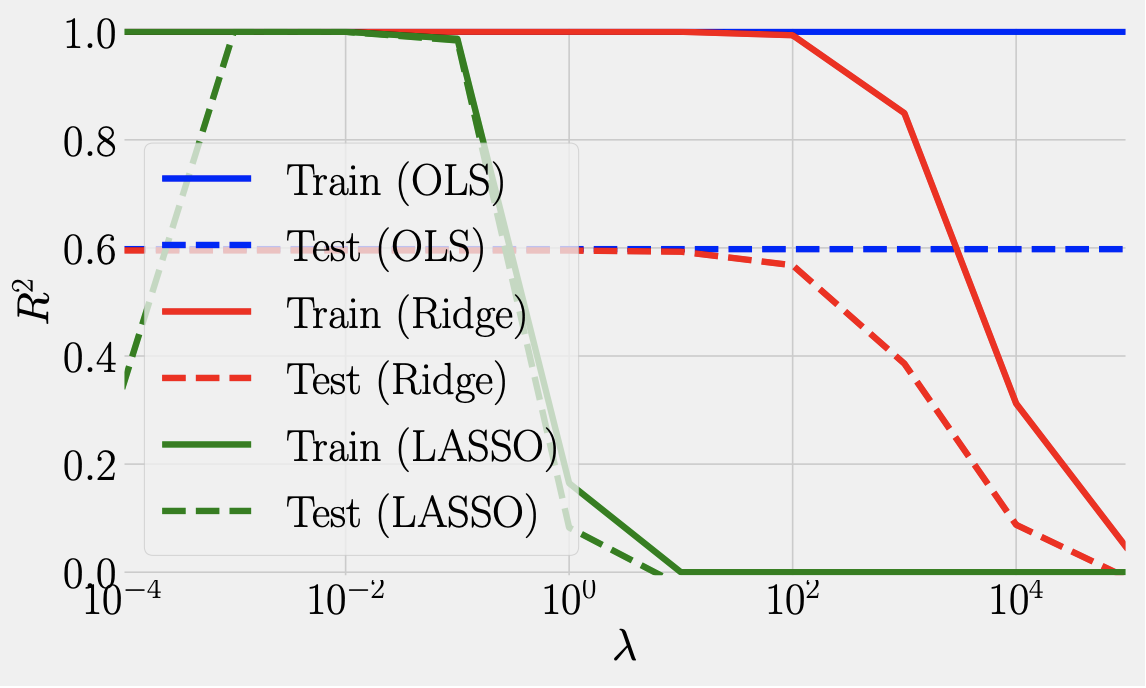
\includegraphics[width = 0.6\paperwidth]{figures/R2_article.png}
\caption{Performance of OLS, Ridge and LASSO regression on the 1D Ising model as measured by the 
    R2 score. Figure 16 in \cite{HighBias}} 
\label{fig:regression-r2-article}

\end{figure}
\subsection{Classifying with Logistic Regression}
To discuss the logistic regression model, 
we look at figure \ref{fig:logistic-eta}. For some $\eta$ the model 
quickly rises to an approximate highest value, but jumps back down to 
the equivalent of guessing.
When approaching 30 epochs and more, this behaviour 
diminishes somewhat, and overall the etas that produce the best results 
($10^{-5} - 10^{-2}$) have most of their values in the higher points.
From table \ref{tab:logistic-critical} we see that the accuracy is best
for \(\eta = 10^{-3}\). Even so, the accuracy is still 
way below 1.0, making this logistic model only marginally better than guessing. 
Table ~\ref{tab:logistic-critical} can be compared to figure 
~\ref{fig:logistic-article}. We see that our model is slightly 
worse than the one described in the article, but that they 
follow a similar trend.

\begin{figure}[H]
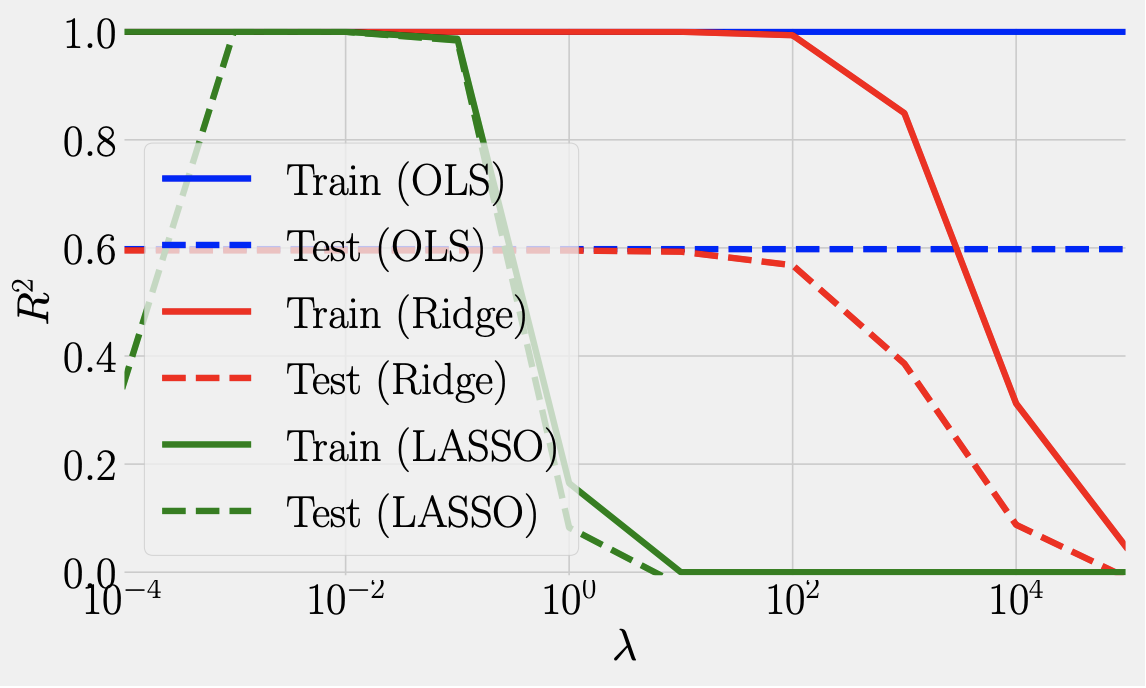
\includegraphics[width = 0.6\paperwidth]{figures/R2_article.png}
\caption{Accuracy as a function of the regularization parameter
\(\lambda\) in classifying the phases of the 2D Ising model on the
training (blue), test (red), and critical (green) data. The solid
and dashed lines compare the ’liblinear’ and ’SGD’ solvers, respectively..Figure 21 in ~\cite{HighBias}} 
\label{fig:logistic-article}
\end{figure}


\subsection{Classifying with Neural Network}
The neural network results in figure \ref{fig:nn-grids} show that the network
performs far better than logistic regression, reaching 1.0 accuracy on both training and
test sets, and as much as 0.97 on the critical set. Adding that the network is trained
on only 10\% of the data that the logistic regressor was applied to, it is significantly better,
and faster.
Note that the network with a more complex architecture, with two layers and far more nodes in 
each layer, doesn't perform better on the data from the critical temperature region. 
This indicates that performance on the test set alone is not a good indicator of how well
the network generalizes. From the grid searches, it also seems that the regularization
parameter plays a larger role for the less complex network.


